% BIDS-Eye project page, Figure 2: evidence tiers on one example question.
% States and the keep rule follow backend/services/uncertain_tier.py (defaults:
% UNCERTAIN_MAX_UNSURE=1, UNCERTAIN_POSSIBLE=false). The five datasets are schematic.
% Build:  ./build-paper-figures.sh
\documentclass[tikz,border=8pt]{standalone}
\usepackage[T1]{fontenc}
\usepackage{lmodern}
\usepackage{textcomp}
\usepackage{amssymb}
\usetikzlibrary{arrows.meta,positioning,calc,backgrounds}

\definecolor{ink}{HTML}{1B1F24}
\definecolor{mute}{HTML}{59616B}
\definecolor{rule}{HTML}{B9BFC7}
\definecolor{conF}{HTML}{E3F3EA} \definecolor{conB}{HTML}{17704C}
\definecolor{proF}{HTML}{FBF0D2} \definecolor{proB}{HTML}{94660A}
\definecolor{posF}{HTML}{EEF0F3} \definecolor{posB}{HTML}{6A727D}
\definecolor{ctrF}{HTML}{FBE6E3} \definecolor{ctrB}{HTML}{B03A2E}

\begin{document}
\hyphenpenalty=10000 \exhyphenpenalty=10000
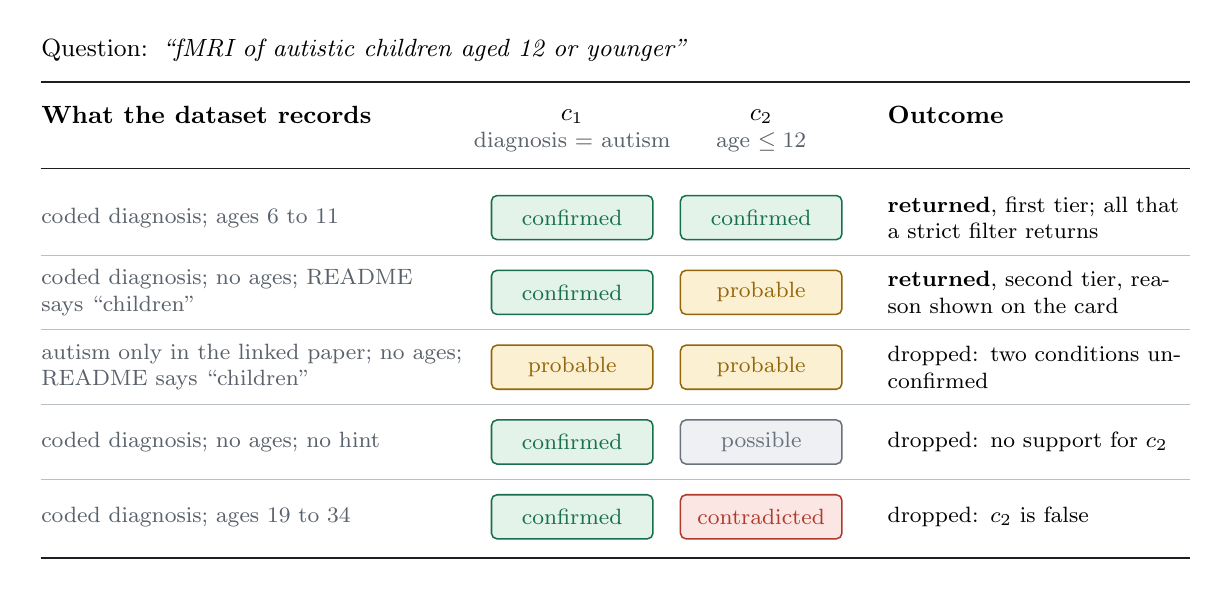
\begin{tikzpicture}[
  font=\small\color{ink},
  show background rectangle, background rectangle/.style={fill=white},
  pill/.style={draw=#1B, fill=#1F, text=#1B, line width=0.55pt, rounded corners=2pt,
               font=\footnotesize, minimum width=2.05cm, minimum height=0.56cm, inner sep=2pt},
  head/.style={font=\small\bfseries, align=center, anchor=south, inner sep=2pt},
  subh/.style={font=\footnotesize\color{mute}, align=center, anchor=north, inner sep=2pt},
  rec/.style={font=\footnotesize\color{mute}, anchor=west, align=left, text width=5.35cm, inner sep=0pt},
  outc/.style={font=\footnotesize, anchor=west, align=left, text width=3.85cm, inner sep=0pt},
]
\def\xa{6.75} \def\xb{9.15} \def\xo{10.75} \def\xr{14.6}

% Question
\node[anchor=west, inner sep=0pt, font=\small] at (0,1.62)
  {Question:\enspace\textit{``fMRI of autistic children aged 12 or younger''}};

% Header
\node[head, anchor=south west, inner xsep=0pt] at (0,0.62) {What the dataset records};
\node[head] at (\xa,0.62) {$c_1$};
\node[subh] at (\xa,0.66) {diagnosis = autism};
\node[head] at (\xb,0.62) {$c_2$};
\node[subh] at (\xb,0.66) {age $\le 12$};
\node[head, anchor=south west, inner xsep=0pt] at (\xo,0.62) {Outcome};
\draw[ink, line width=0.8pt] (0,1.22) -- (\xr,1.22);
\draw[ink, line width=0.45pt] (0,0.12) -- (\xr,0.12);

% Rows: y, record, state c1, state c2, outcome
\foreach \y/\r/\sa/\la/\sb/\lb/\o in {
  -0.50/{coded diagnosis; ages 6 to 11}/con/confirmed/con/confirmed/{\textbf{returned}, first tier; all that a strict filter returns},
  -1.45/{coded diagnosis; no ages; README says ``children''}/con/confirmed/pro/probable/{\textbf{returned}, second tier, reason shown on the card},
  -2.40/{autism only in the linked paper; no ages; README says ``children''}/pro/probable/pro/probable/{dropped: two conditions unconfirmed},
  -3.35/{coded diagnosis; no ages; no hint}/con/confirmed/pos/possible/{dropped: no support for $c_2$},
  -4.30/{coded diagnosis; ages 19 to 34}/con/confirmed/ctr/contradicted/{dropped: $c_2$ is false}}
{
  \node[rec] at (0,\y) {\r};
  \node[pill=\sa] at (\xa,\y) {\la};
  \node[pill=\sb] at (\xb,\y) {\lb};
  \node[outc] at (\xo,\y) {\o};
}
\foreach \y in {-0.975,-1.925,-2.875,-3.825}
  \draw[rule, line width=0.35pt] (0,\y) -- (\xr,\y);
\draw[ink, line width=0.8pt] (0,-4.82) -- (\xr,-4.82);

\end{tikzpicture}
\end{document}
